% -*- TeX-master: "sbml-level-3-version-2-core"; fill-column: 66 -*-
% ----------------------------------------------------------------

\section{A method for assessing whether an SBML model is overdetermined}
\label{apdx:assessing-overdetermined}

As explained in Section~\ref{sec:ruleconstraints}, an SBML model
must not be overdetermined.  It is possible to use purely static
analysis to assess this condition for the system of equations implied by a
model, by constructing a bipartite graph of the model's variables
and equations and then searching for a maximal
matching~\citep{chartrand_1977}.  An efficient algorithm for finding
a maximal matching is described by \cite{hopcroft:1973}.  In this
appendix, we provide a concrete application to SBML of the general
approach described in Section~\ref{sec:ruleconstraints}.  The
approach is defined in terms of the ordinary differential
equations (ODEs) implied by an SBML model; 
despite our use of a differential equation framework for
  this explanation, it should be understood that this
use of ODEs has no implication about the framework
  actually used to simulate the model.


\subsection*{Definition of the method}
\label{sec:overdetermined-method}

First, we assume that an ODE is constructed for each species
determined by one or more \Reaction's \KineticLaw \token{math}
expressions.  We also assume that the model has already been
determined to be valid in all other respects (\eg there are no
undefined variables in the equations), and what remains is to
evaluate whether it is overdetermined.

We construct the bipartite graph for a given SBML model as follows:
\begin{enumerate}

\item For each of the following in the model, create one vertex
  representing an equation:
  \begin{enumerate}
    
  \item Every \Species object having
    \token{boundaryCondition}=\val{false},
    \token{constant}=\val{false}, and which is referenced as a
    reactant or product in one or more \Reaction objects
    containing \KineticLaw objects

  \item Every \AssignmentRule object

  \item Every \RateRule object

  \item Every \AlgebraicRule object

  \item Every \KineticLaw object

  \end{enumerate}
  
\item For each of the following in the model, create one vertex
  representing a variable:
  \begin{enumerate}

  \item Every \Species object having \token{constant}=\val{false}
  \item Every \Compartment object having \token{constant}=\val{false}
  \item Every global \Parameter having \token{constant}=\val{false}
  \item Every \SpeciesReference object having \token{constant}=\val{false}
  \item Every \Reaction object

  \end{enumerate}
  
\item For each of the following, create one edge:
  \begin{enumerate}
    
  \item Every vertex created in step 2(a) to that species'
    equation vertex created in step 1(a)
    
  \item Every vertex created in step 1(b) to the particular vertex
    created in steps 2(a)--2(e) that represents the variable
    referenced by the \token{variable} attribute of the rule
    
  \item Every vertex created in step 1(c) to the particular vertex
    created in steps 2(a)--2(e) that represents the variable
    referenced by the \token{variable} attribute of the rule
    
  \item Every vertex created in step 1(e) to the particular vertex
    created in step 2(e) that is the \Reaction object containing
    that particular \KineticLaw object
    
  \item Every vertex created in steps 2(a)--2(e) representing an
    identifier appearing as the content of a MathML \token{ci}
    element within an expression of an \AlgebraicRule, to the
    vertex for that particular \AlgebraicRule created in step 1(d)
    
  \end{enumerate}

\end{enumerate}


\subsection*{Example application of the method}

What follows is an example of applying the method above to the
SBML model shown below:

\sbmlexample{overdetermined.xml}

For the model above, we create \emph{equation} vertices as
follows:
\begin{enumerate}\setlength{\parskip}{0.2ex}
  
\item{} [Corresponding to step 1(a) in
  Section~\ref{sec:overdetermined-method}.]  \emph{Every \Species
    object having \token{boundaryCondition}=\val{false},
    \token{constant}=\val{false}, and which is referenced as a
    reactant or product in one or more \Reaction objects
    containing \KineticLaw objects}.  This generates two vertices,
  for \val{S1} and \val{S2}.
  
\item{} [Corresponding to step 1(b)
  in Section~\ref{sec:overdetermined-method}.] \emph{Every
    \AlgebraicRule object}.  This generates one vertex, for the
  model's lone algebraic rule (call it \val{rule}).
  
\item{} [Corresponding to step 1(e)
  in Section~\ref{sec:overdetermined-method}.] \emph{Every \KineticLaw
    object}.  This generates one vertex, for the lone kinetic law
  in the model (call it \val{law}).

\end{enumerate}

\clearpage
We create \emph{variable} vertices for the following:
\begin{enumerate}
  
\item{} [Corresponding to step 2(a)
  in Section~\ref{sec:overdetermined-method}.] \emph{Every \Species
    object having \token{constant}=\val{false}}.  This generates
  two vertices, for \val{S1} and \val{S2}.
  
\item{} [Corresponding to step 2(e)
  in Section~\ref{sec:overdetermined-method}.] \emph{Every \Reaction
    object}.  This generates one vertex, for \val{R}.

\end{enumerate}

Note that it is not necessary to include parameters declared
within \KineticLaw objects because they are local to a particular
reaction and cannot be affected by rules.  With the steps above,
we have the following set of graph nodes:
\begin{center}
\emph{Vertices for equations}\\[10pt]
  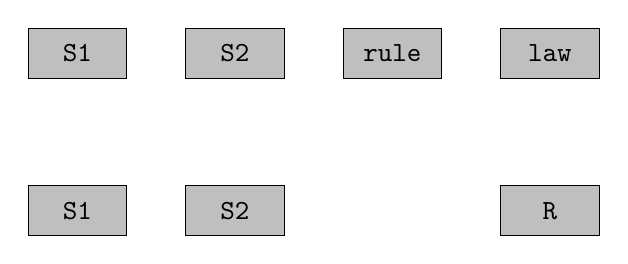
\begin{tikzpicture}
    \tikzstyle{every node}=[draw, fill=lightgray, text centered,
    text width=0.4in, minimum height=0.25in, font=\ttfamily]

    \node (a) at (-3, 1) {S1};
    \node (b) at (-1, 1) {S2};
    \node (c) at ( 1, 1) {rule};
    \node (d) at ( 3, 1) {law};

    \node (e) at (-3,-1) {S1};
    \node (f) at (-1,-1) {S2};
%    \node (g) at ( 1,-1) {C};
    \node (h) at ( 3,-1) {R};
  \end{tikzpicture}\\[5pt]
\emph{Vertices for variables}
\end{center}

Next, we create edges following the procedure described above.
Doing so results in the following graph:
\begin{center}
\emph{Vertices for equations}\\[10pt]
  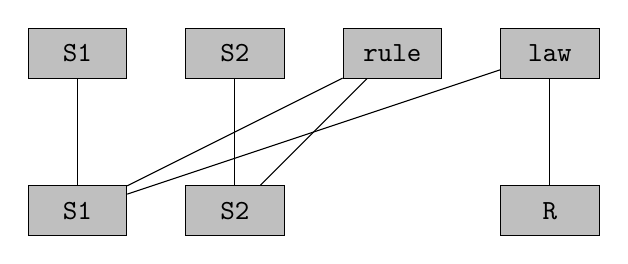
\begin{tikzpicture}
    \tikzstyle{every node}=[draw, fill=lightgray, text centered,
    text width=0.4in, minimum height=0.25in, font=\ttfamily]

    \node (a) at (-3, 1) {S1};
    \node (b) at (-1, 1) {S2};
    \node (c) at ( 1, 1) {rule};
    \node (d) at ( 3, 1) {law};

    \node (e) at (-3,-1) {S1};
    \node (f) at (-1,-1) {S2};
%    \node (g) at ( 1,-1) {C};
    \node (h) at ( 3,-1) {R};

    \draw[shorten <=0pt,shorten >=0pt] (a) -- (e);
    \draw[shorten <=0pt,shorten >=0pt] (b) -- (f);
    \draw[shorten <=0pt,shorten >=0pt] (c) -- (e);
    \draw[shorten <=0pt,shorten >=0pt] (c) -- (f);
    \draw[shorten <=0pt,shorten >=0pt] (d) -- (e);
    \draw[shorten <=0pt,shorten >=0pt] (d) -- (h);
  \end{tikzpicture}\\[5pt]
\emph{Vertices for variables}
\end{center}

The algorithm of \cite{hopcroft:1973} can now be applied to search
for a maximal matching of the bipartite graph.  A maximal matching
is a graph in which each vertex is connected to at most one other
vertex and the maximum possible number of connections have been
made.  Doing so here results in the following:
\begin{center}
\emph{Vertices for equations}\\[10pt]
  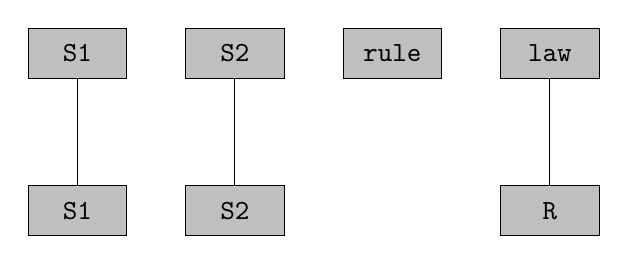
\begin{tikzpicture}
    \tikzstyle{every node}=[draw, fill=lightgray, text centered,
    text width=0.4in, minimum height=0.25in, font=\ttfamily]

    \node (a) at (-3, 1) {S1};
    \node (b) at (-1, 1) {S2};
    \node (c) at ( 1, 1) {rule};
    \node (d) at ( 3, 1) {law};

    \node (e) at (-3,-1) {S1};
    \node (f) at (-1,-1) {S2};
%    \node (g) at ( 1,-1) {C};
    \node (h) at ( 3,-1) {R};

    \draw[shorten <=0pt,shorten >=0pt] (a) -- (e);
    \draw[shorten <=0pt,shorten >=0pt] (b) -- (f);
    \draw[shorten <=0pt,shorten >=0pt] (d) -- (h);
  \end{tikzpicture}\\[5pt]
\emph{Vertices for variables}
\end{center}

If the maximal matching of the bipartite graph leaves any equation
vertex unconnected, then the model is considered overdetermined.
That is the case for the example shown here, because the equation
vertex for \val{rule} is unconnected in the maximal matching.


